% Set the author and title of the compiled pdf
\hypersetup{
  pdftitle = {\Title},
  pdfauthor = {\Author}
}

\section{A history of software engineering}

In the 60's, when programming projects started to get large enough to warrant
their own software develoment strategies. The increased complexity of projects
at this time was leading to many of them going over budget, over time, having
low quality, not meeting requirements, and being difficult to maintain. This,
even at the time, was refferred to as the software crisis.

Dijkstra summed it up in an article in Communications of the ACM:

\begin{aquote}{Dijkstra}
  The major cause of the software crisis is that the machines have become
  several orders of magnitude more powerful! To put it quite bluntly: as long
  as there were no machines, programming was no problem at all; when we had a
  few weak computers, programming became a mild problem, and now we have
  gigantic computers, programming has become an equally gigantic problem.
\end{aquote}

\subsection{Why do projects fail?}

We've seen that projects often failed early on in the history of software
development, but why did each project fail? There are a large number of
reasons why a specific project could end in failiure, however, there also a
number of common reasons for disaster:

\begin{itemize}
  \item Unrealistic goals
  \item Inaccurate estimate of project complexity/resources needed
  \item Badly defined requirements
  \item Unmanaged risk
  \item Use of immature technology
  \item Sloppy devevlopment practices
\end{itemize}

Now, there are software development practices and methodologies that aim to
mitigate the risk of project failiure by defining how a project should be
developed. Figure~\ref{fig:gen-software-dev-process} shows the a generic view
of such a process.

\begin{figure}[!h]
  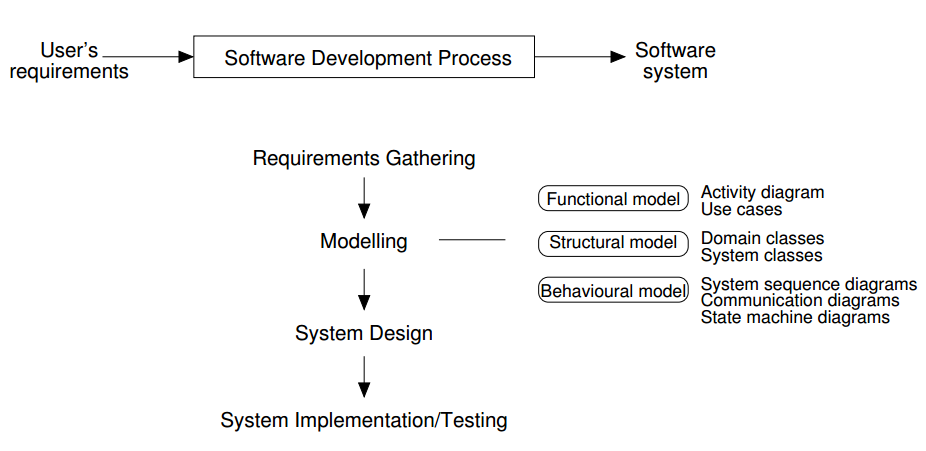
\includegraphics[width=\textwidth]{images/generic-software-dev-process.jpg}
  \label{fig:gen-software-dev-process}
  \caption{A generic software development process}
\end{figure}

\section{Gathering requirements}

Gathering the requirements of a software project is crucial, since if a
developer doesn't understand what is being created, how can they create it
properly? There are two types of requirements, functional and non functional.

\textbf{Functional} requirements are things that the system should textbf{do}.
For example, the system should produce both a a4 sized document, and a a5
sized e-readable copy.

\textbf{Non Functional} requirements are things the system should \textbf{be}.
This could be that the system should be developed with ethical software
development practices, or the system should be easily extensible for future
development.

When gathering the requirements of the process, it is important to accurately
capture the buisiness process that is being encapsulated in the system. It is
important to understand the state of the process now, and the desired state of
the process at the end of the development time. UML is a way of representing
buisiness logic, and the relationship between differnt parts of the system.
Activity diagrams can be used to create a logical model of the system.

\textit{Activities} are composed of \textit{actions}, which are non-
decomposable pieces of behaviour. Activity diagrams are composed of
activities.
